\documentclass[border=0.8ex,svgnames,tikz]{standalone}
\usepackage{amsmath,mathtools}
\usepackage{fontspec}
\setmainfont{Source Serif 4}
\setsansfont{Source Sans 3}
\setmonofont{Source Code Pro}
\usetikzlibrary{arrows.meta}
\begin{document}
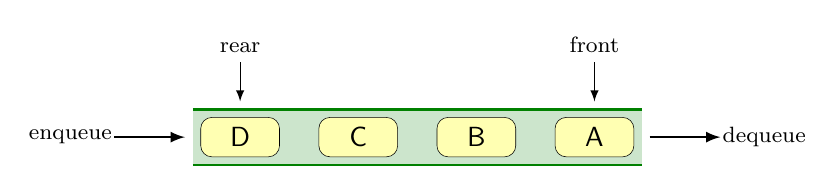
\begin{tikzpicture}[
  queue element/.style={
    draw,
    very thin,
    rounded corners,
    fill=Yellow!30,
    minimum width=1cm,
    minimum height=.5cm,
    font=\sffamily,
  },
  >=latex,
  ]
  \path[fill=Green!20] (5.1,.35) rectangle (-.6,-.35);
  \path[draw=Green,thick] (-.6,+.35) -- (5.1,+.35) (-.6,-.35) -- (5.1,-.35);
  \foreach \i/\name in {0/D,1/C,2/B,3/A} {
    \node[queue element] (\name) at (1.5*\i,0) {\name};
  };
  \path[draw,<-] ([yshift=.2cm]A.north) -- ++(0,.5)
  node[above,font=\footnotesize]{front};
  \path[draw,<-] ([yshift=.2cm]D.north) -- ++(0,.5)
  node[above,font=\footnotesize]{rear};
  \path[draw,->,thick] (5.2,0) to +(.9,0) node[right,font=\footnotesize,inner
  sep=0.1ex]{dequeue};
  \path[draw,->,thick] (-.7,0) +(-.9,0) node[left,font=\footnotesize,inner sep=0.1ex]{enqueue} to (-.7,0);
\end{tikzpicture}
\end{document}
